% ============================================================
%  PhD Defense — AI-Powered Educational Crossword Generation
%  Tommaso Iaquinta · Università di Siena
% ============================================================
\documentclass[aspectratio=169, 12pt]{beamer}

% ---- Theme ----
\usetheme{default}
\usecolortheme{default}

% ---- Colors (University of Siena palette) ----
\definecolor{unisired}{RGB}{140, 15, 25}
\definecolor{darktext}{RGB}{40, 40, 40}
\definecolor{graytext}{RGB}{110, 110, 110}
\definecolor{lightbg}{RGB}{248, 248, 248}
\definecolor{accentblue}{RGB}{0, 90, 150}

\setbeamercolor{structure}{fg=unisired}
\setbeamercolor{frametitle}{fg=unisired, bg=white}
\setbeamercolor{title}{fg=white}
\setbeamercolor{subtitle}{fg=white!85}
\setbeamercolor{author}{fg=white!80}
\setbeamercolor{date}{fg=white!70}
\setbeamercolor{block title}{fg=white, bg=unisired}
\setbeamercolor{block body}{bg=lightbg}
\setbeamercolor{item}{fg=unisired}
\setbeamercolor{footline}{fg=graytext, bg=white}
\setbeamercolor{normal text}{fg=darktext}
\setbeamercolor{section in toc}{fg=unisired}

% ---- Navigation off ----
\setbeamertemplate{navigation symbols}{}

% ---- Footline ----
\setbeamertemplate{footline}{%
  \leavevmode%
  \hbox{%
    \begin{beamercolorbox}[wd=.33\paperwidth,ht=2.25ex,dp=1ex,left]{footline}%
      \hspace{1em}{\small T.\ Iaquinta}%
    \end{beamercolorbox}%
    \begin{beamercolorbox}[wd=.33\paperwidth,ht=2.25ex,dp=1ex,center]{footline}%
      {\small PhD Defense — 2026}%
    \end{beamercolorbox}%
    \begin{beamercolorbox}[wd=.33\paperwidth,ht=2.25ex,dp=1ex,right]{footline}%
      {\small\insertframenumber\,/\,\inserttotalframenumber}\hspace{1em}%
    \end{beamercolorbox}%
  }%
  \vskip2pt%
}

% ---- Frame title with red rule ----
\setbeamertemplate{frametitle}{%
  \vskip0.5em%
  \usebeamerfont{frametitle}\insertframetitle%
  \vskip-0.15em%
  {\color{unisired}\rule{\textwidth}{0.5pt}}%
  \vskip0.2em%
}

% ---- Fonts ----
\usefonttheme{professionalfonts}
\setbeamerfont{title}{size=\Large, series=\bfseries}
\setbeamerfont{subtitle}{size=\normalsize}
\setbeamerfont{frametitle}{size=\large, series=\bfseries}

% ---- Items ----
\setbeamertemplate{itemize items}[circle]
\setbeamertemplate{enumerate items}[default]

% ---- Section page ----
\AtBeginSection[]{%
  {%
    \setbeamertemplate{footline}{}%
    \setbeamercolor{background canvas}{bg=unisired}%
    \begin{frame}[plain]
      \vfill
      \begin{center}
        {\fontsize{28}{34}\selectfont\color{white}\textbf{\insertsectionhead}}
      \end{center}
      \vfill
    \end{frame}
  }%
}

% ---- Packages ----
\usepackage[utf8]{inputenc}
\usepackage[T1]{fontenc}
\usepackage{graphicx}
\usepackage{booktabs}
\usepackage{tikz}
\usetikzlibrary{shapes, arrows.meta, positioning, calc, decorations.pathreplacing}
\usepackage{amsmath, amssymb}
\usepackage{hyperref}
\usepackage{multicol}

% ---- Meta ----
\title{AI-Powered Educational Crossword Generation}
\subtitle{From Linguistic Resources to Adaptive Gamified Learning}
\author{Tommaso Iaquinta}
\institute{Universit\`a di Siena\\ Dottorato in Computer Science and Engineering}
\date{2026}


\begin{document}

% ======================================================
%  TITLE
% ======================================================
{
\setbeamertemplate{footline}{}
\setbeamercolor{background canvas}{bg=unisired}
\begin{frame}[plain]
  \vfill
  \begin{columns}[c]
    \column{0.13\textwidth}
      \centering
      
\includegraphics[width=0.95\textwidth]{figures/sigillo.png}
    \column{0.87\textwidth}
      {\usebeamerfont{title}\usebeamercolor[fg]{title}\inserttitle}\\[0.6em]
      {\usebeamerfont{subtitle}\usebeamercolor[fg]{subtitle}\insertsubtitle}\\[1.8em]
      {\usebeamercolor[fg]{author}\insertauthor}\\[0.3em]
      {\usebeamercolor[fg]{date}\small\insertinstitute}\\[0.3em]
      {\usebeamercolor[fg]{date}\small\insertdate}
  \end{columns}
  \vfill
\end{frame}
}

% ======================================================
%  OUTLINE
% ======================================================
\begin{frame}{Roadmap}
  \tableofcontents[hideallsubsections]
\end{frame}

% ======================================================
%  1 — MOTIVATION
% ======================================================
\section{Why AI + Crosswords in Education?}

% --- 1.1 History timeline ---
\begin{frame}{Technology Has Never ``Revolutionized'' Education}
  \begin{center}
    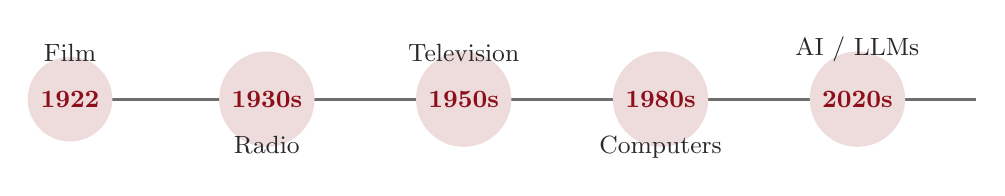
\begin{tikzpicture}[
      yearnode/.style={circle, fill=unisired!15, minimum size=1cm, font=\small\bfseries, text=unisired},
      technode/.style={font=\small, text=darktext, align=center},
    ]
    \draw[line width=1pt, graytext] (0,0) -- (12,0);
    \node[yearnode] at (0.5, 0) {1922};
    \node[technode, above=0.35cm] at (0.5, 0) {Film};
    \node[yearnode] at (3, 0) {1930s};
    \node[technode, below=0.35cm] at (3, 0) {Radio};
    \node[yearnode] at (5.5, 0) {1950s};
    \node[technode, above=0.35cm] at (5.5, 0) {Television};
    \node[yearnode] at (8, 0) {1980s};
    \node[technode, below=0.35cm] at (8, 0) {Computers};
    \node[yearnode] at (10.5, 0) {2020s};
    \node[technode, above=0.35cm] at (10.5, 0) {AI / LLMs};
    \end{tikzpicture}
  \end{center}
  \vfill
  \begin{quote}
    \small\color{graytext}%
    ``The motion picture is destined to revolutionize our educational system
    and [\ldots] supplant the use of textbooks.''\\
    \upshape\hfill --- \textbf{Thomas Edison, 1922}
  \end{quote}
  \vspace{0.3em}
  \centering{\small Spoiler: it didn't.}
\end{frame}

% --- 1.2 AI evidence ---
\begin{frame}{Yet AI \textit{Does} Improve Learning}
  \begin{columns}[c]
    \column{0.5\textwidth}
      \begin{center}
        {\fontsize{56}{66}\selectfont\color{unisired}\textbf{+0.87}}\\[0.3em]
        {\large standard deviations}\\[0.5em]
        {\small\color{graytext} $\approx$ from 50th to \textbf{80th percentile}}
      \end{center}
    \column{0.5\textwidth}
      \small
      Meta-analysis of \textbf{51 studies}\\
      (Nov 2022 -- Feb 2025)\\[1em]
      Students using ChatGPT showed\\
      \textbf{large positive effects} on\\
      learning performance.\\[1em]
      {\scriptsize\color{graytext} Wang et al.\ (2025), Hedges' $g = 0.867$}
  \end{columns}
\end{frame}

% --- 1.3 Gamification evidence ---
\begin{frame}{Gamification: Small Effort, Real Results}
  \begin{columns}[c]
    \column{0.55\textwidth}
      \begin{center}
        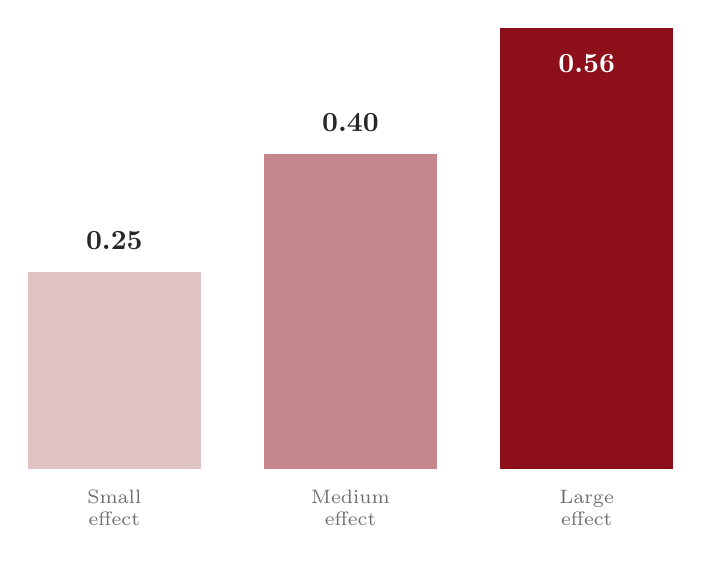
\begin{tikzpicture}
          \fill[unisired!25] (0, 0) rectangle (2.2, 2.5);
          \fill[unisired!50] (3, 0) rectangle (5.2, 4);
          \fill[unisired]     (6, 0) rectangle (8.2, 5.6);
          \node[font=\bfseries, text=darktext] at (1.1, 2.9) {0.25};
          \node[font=\bfseries, text=darktext] at (4.1, 4.4) {0.40};
          \node[font=\bfseries, text=white]    at (7.1, 5.15) {0.56};
          \node[font=\scriptsize, text=graytext, align=center] at (1.1, -0.5) {Small\\effect};
          \node[font=\scriptsize, text=graytext, align=center] at (4.1, -0.5) {Medium\\effect};
          \node[font=\scriptsize, text=graytext, align=center] at (7.1, -0.5) {Large\\effect};
        \end{tikzpicture}
      \end{center}
    \column{0.45\textwidth}
      \small
      Effect sizes from two\\
      large meta-analyses: \textbf{$d = 0.25$--$0.56$}\\[1em]
      Improvements in:\\[0.3em]
      \begin{itemize}
        \item Knowledge retention
        \item Engagement \& persistence
        \item Class participation
      \end{itemize}
      \vspace{0.5em}
      {\scriptsize\color{graytext} Sailer \& Homner (2020); Y\i ld\i r\i m \& \c{S}en (2021)}
  \end{columns}
\end{frame}

% --- 1.4 Why crosswords ---
\begin{frame}{Why Crosswords?}
  \begin{columns}[c]
    \column{0.55\textwidth}
      \small
      Crosswords combine \textbf{multiple cognitive processes}:
      \vspace{0.5em}
      \begin{itemize}
        \setlength\itemsep{0.6em}
        \item \textbf{Active recall} --- each clue triggers retrieval
        \item \textbf{Contextual learning} --- clues embed meaning
        \item \textbf{Self-assessment} --- gaps become visible
        \item \textbf{Engagement} --- the puzzle \textit{is} the reward
      \end{itemize}
      \vspace{0.5em}
      {\scriptsize\color{graytext} Saxena et al.\ (2009); Patrick et al.\ (2018)}
    \column{0.45\textwidth}
      \centering
      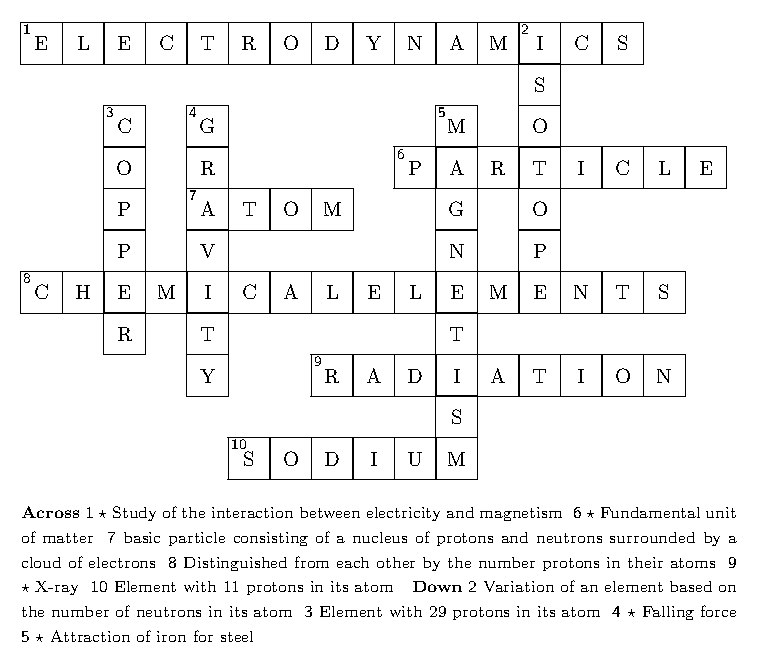
\includegraphics[width=0.85\textwidth]{figures/crossword.pdf}
  \end{columns}
\end{frame}

% --- 1.5 Our goal ---
\begin{frame}{Our Goal}
  \begin{center}
    \vspace{1em}
    
\begin{tikzpicture}[
      box/.style={draw=unisired, rounded corners=8pt, minimum width=3.2cm, minimum height=1.5cm, align=center, font=\small\bfseries, text=unisired, line width=1pt},
      arr/.style={->, >=Stealth, line width=1.5pt, unisired!50}
    ]
    \node[box] (ai) at (0, 0) {Large Language\\Models};
    \node[box] (cross) at (5, 0) {Crossword\\Puzzles};
    \node[box] (edu) at (10, 0) {Educational\\Impact};
    \draw[arr] (ai) -- node[above, font=\scriptsize, text=graytext]{generate} (cross);
    \draw[arr] (cross) -- node[above, font=\scriptsize, text=graytext]{enhance} (edu);
    \end{tikzpicture}
    \vspace{2em}

    {\large An \textbf{end-to-end system} that automatically creates\\[0.3em]
    educational crosswords from text or keywords}
  \end{center}
\end{frame}


% ======================================================
%  2 — DATASET
% ======================================================
\section{The Dataset: 125,600 Italian Clue--Answer Pairs}

% --- 2.1 Overview ---
\begin{frame}{Building a Large-Scale Linguistic Resource}
  \begin{columns}[c]
    \column{0.42\textwidth}
      \begin{center}
        {\fontsize{44}{52}\selectfont\color{unisired}\textbf{125,600}}\\[0.3em]
        {\large unique clue--answer pairs}\\[1.5em]
        {\normalsize\color{graytext} Sources:}\\[0.3em]
        {\small Dizy.com, Cruciverba.it,\\
        La Settimana Enigmistica,\\
        La Repubblica}
      \end{center}
    \column{0.58\textwidth}
      \centering
      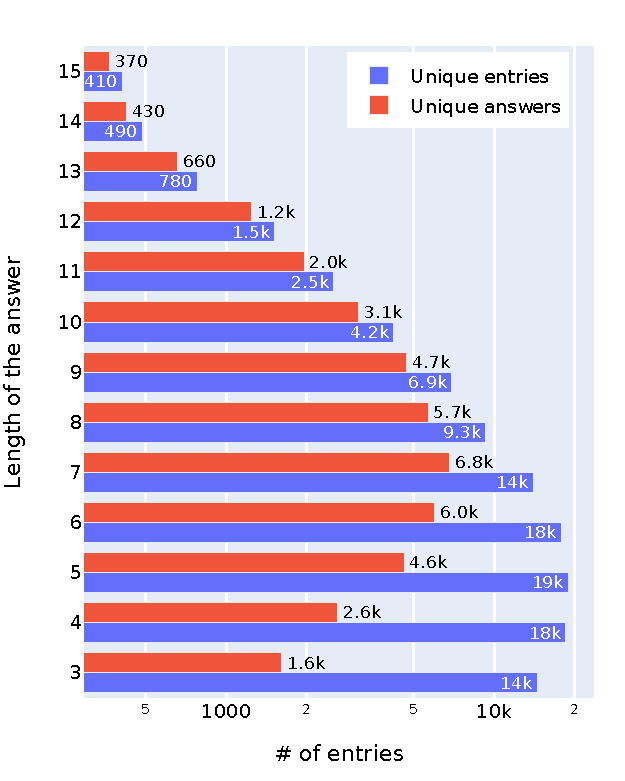
\includegraphics[width=\textwidth]{figures/italian_db.pdf}
  \end{columns}
  \vfill
  {\scriptsize\color{graytext} Publicly available:
  \url{https://github.com/tommyiaq/cruciverba} --- CC BY-NC 4.0}
\end{frame}

% --- 2.2 Linguistic typology ---
\begin{frame}{Linguistic Typology: 20+ Clue Structures}
  \begin{columns}[c]
    \column{0.5\textwidth}
      \small
      Systematic syntactic analysis\\
      via spaCy dependency parsing.\\[1em]
      \textbf{20+ distinct structures} identified:
      \vspace{0.5em}
      \begin{itemize}
        \setlength\itemsep{0.4em}
        \item Nominal phrases (definitions)
        \item Adjectival / prepositional phrases
        \item Copular statements (``X is Y'')
        \item Active / passive verb clauses
        \item Imperative, infinitive, relative clauses
      \end{itemize}
    \column{0.5\textwidth}
      \centering
      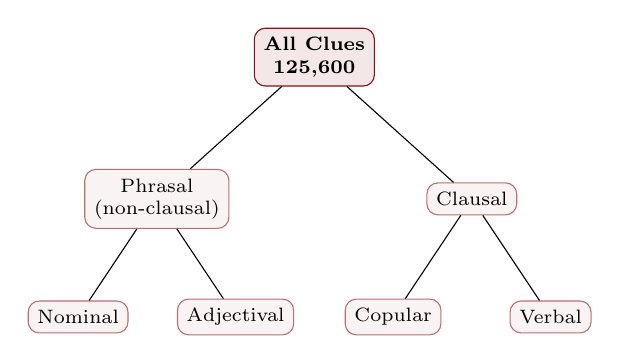
\begin{tikzpicture}[
        level 1/.style={sibling distance=4cm, level distance=1.8cm},
        level 2/.style={sibling distance=2cm, level distance=1.5cm},
        every node/.style={font=\scriptsize, align=center},
        root/.style={draw=unisired, rounded corners, fill=unisired!10, font=\scriptsize\bfseries},
        cat/.style={draw=unisired!60, rounded corners, fill=unisired!5}
      ]
      \node[root] {All Clues\\125,600}
        child {node[cat] {Phrasal\\(non-clausal)}
          child {node[cat] {Nominal}}
          child {node[cat] {Adjectival}}
        }
        child {node[cat] {Clausal}
          child {node[cat] {Copular}}
          child {node[cat] {Verbal}}
        };
      \end{tikzpicture}
      \vspace{0.5em}

      {\scriptsize\color{graytext} Hierarchical taxonomy based\\on generative grammar principles}
  \end{columns}
\end{frame}


% ======================================================
%  3 — ARCHITECTURE
% ======================================================
\section{System Architecture}

% --- 3.1 Pipeline overview ---
\begin{frame}{The Pipeline at a Glance}
  \begin{center}
    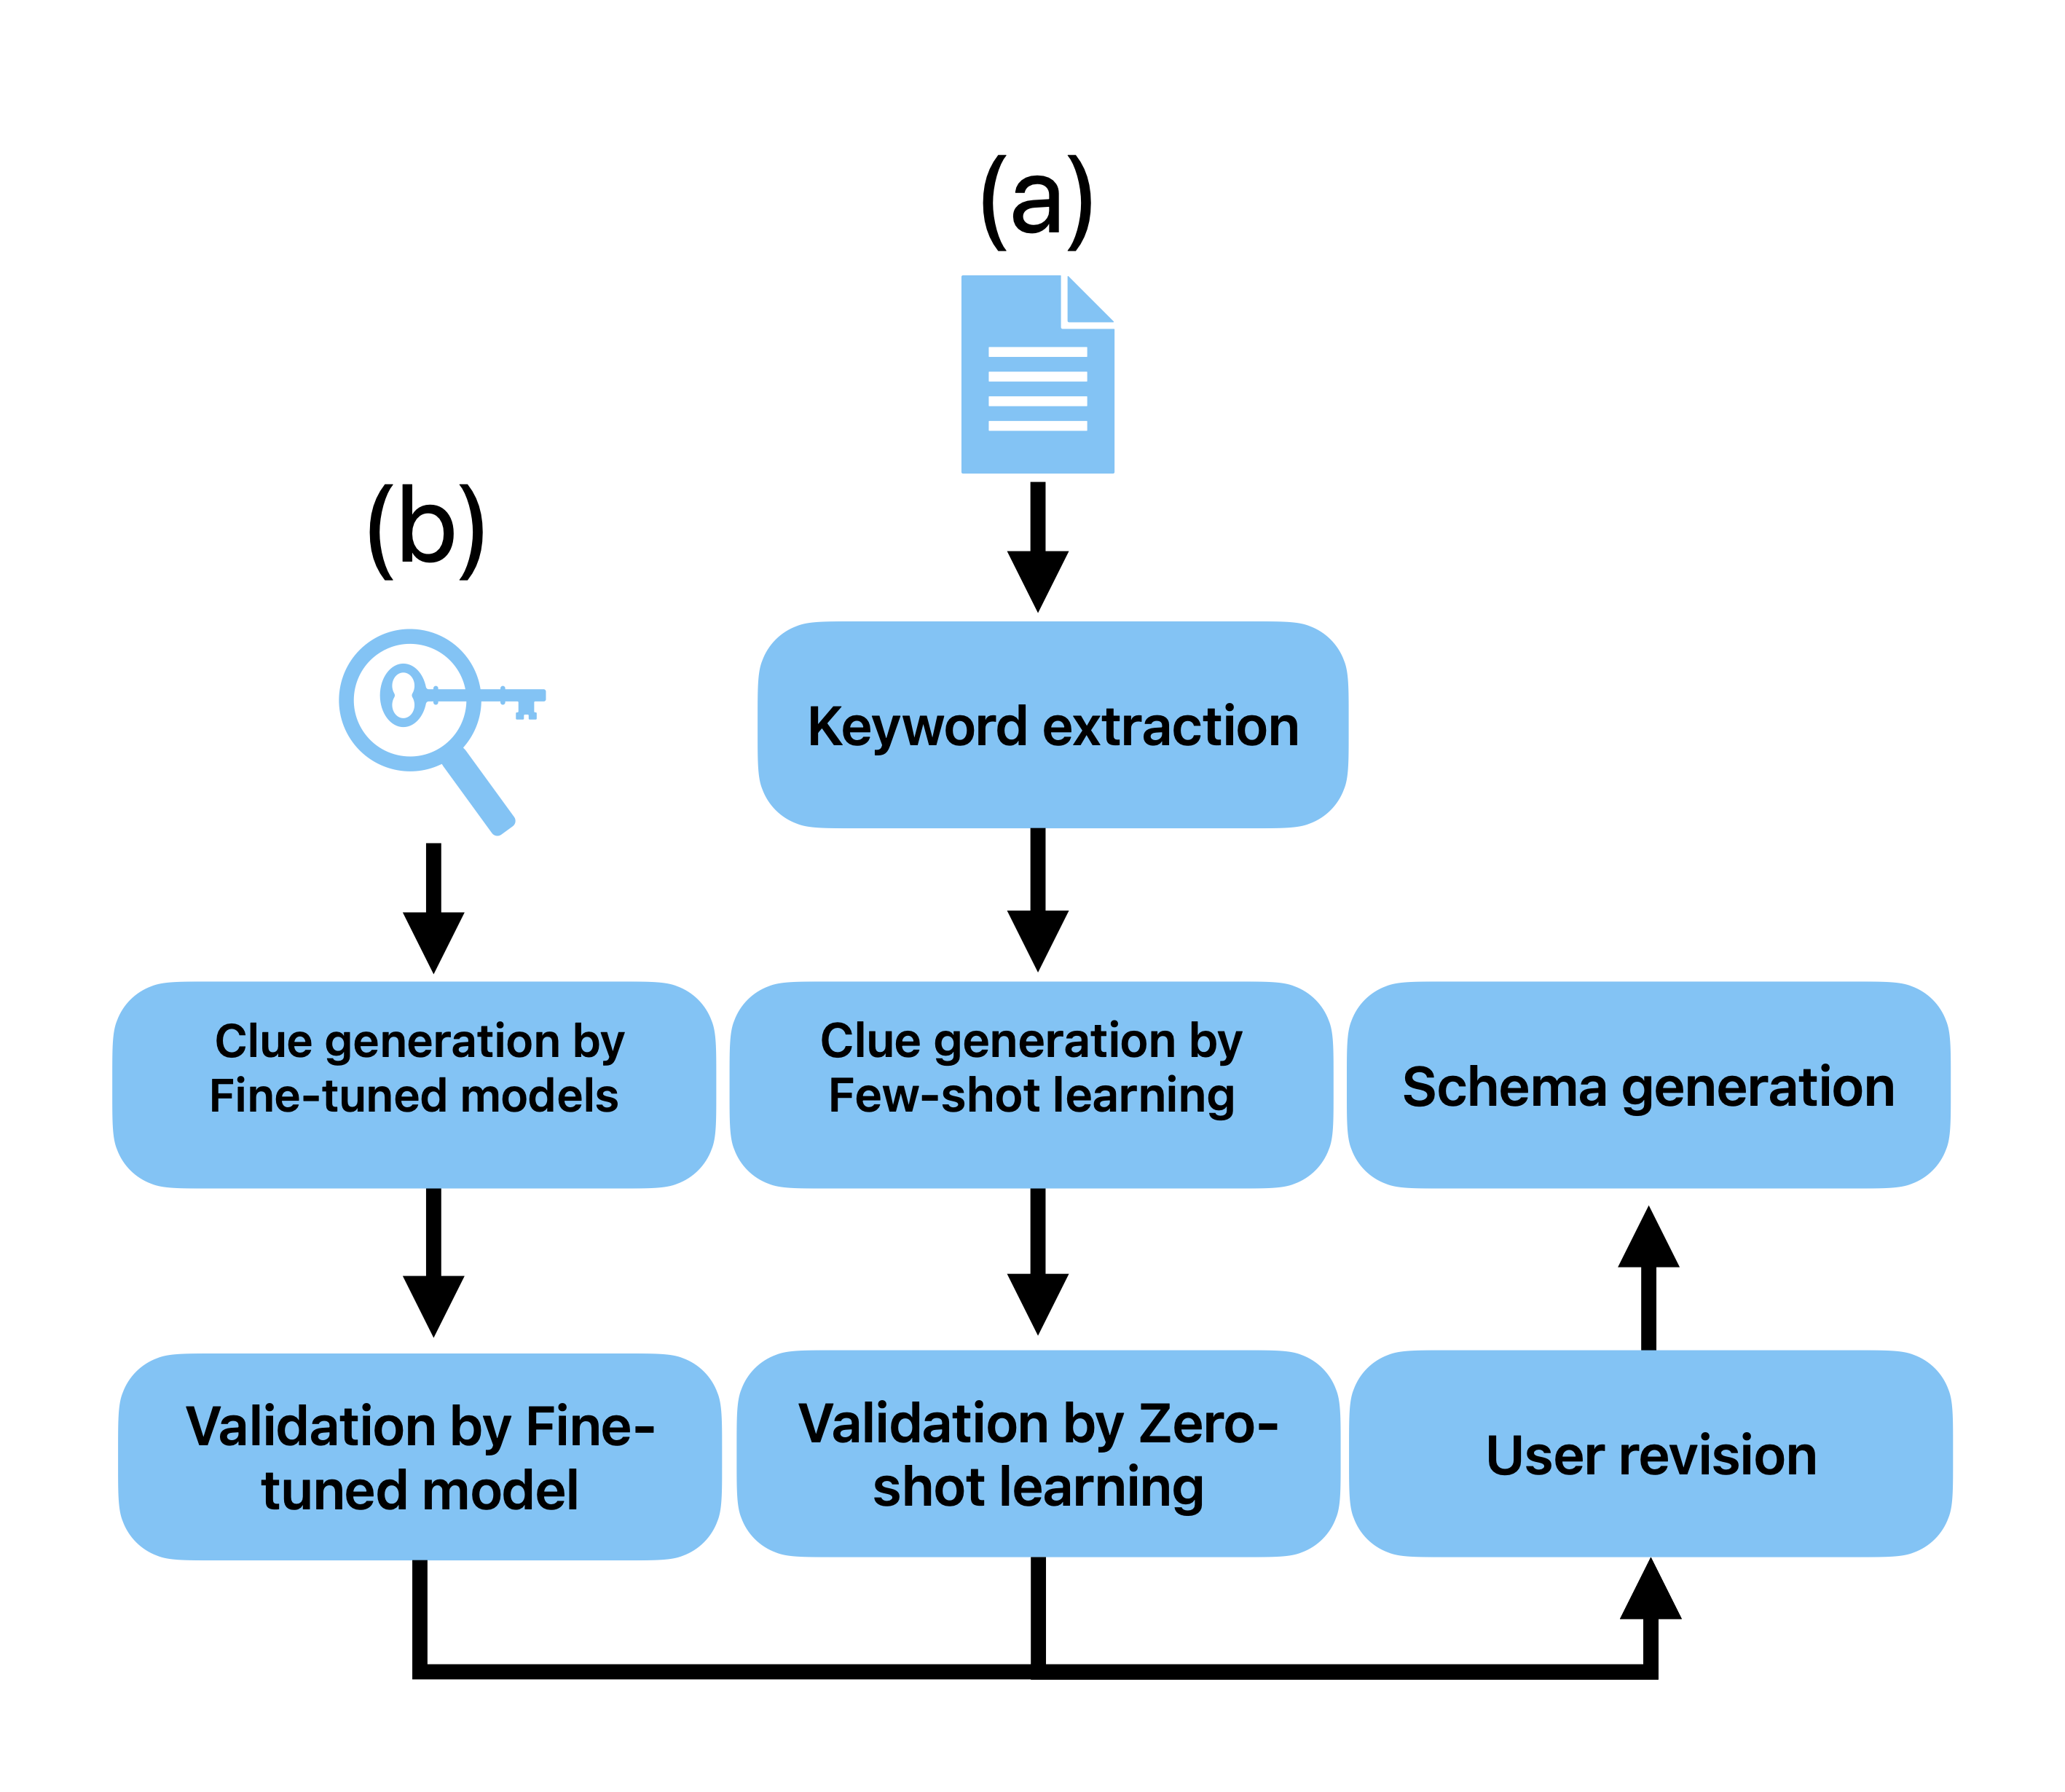
\includegraphics[width=0.82\textwidth]{figures/fig2.png}
  \end{center}
  \vspace{0.5em}
  \begin{columns}[t]
    \column{0.45\textwidth}
      \centering
      {\small\textbf{Path (a)}: Text $\rightarrow$ Keywords $\rightarrow$ Clues}
    \column{0.45\textwidth}
      \centering
      {\small\textbf{Path (b)}: Keywords $\rightarrow$ Clues}
  \end{columns}
  \vspace{0.3em}
  \centering{\small\color{graytext} Both paths converge into validation, human revision, and grid assembly.}
\end{frame}

% --- 3.2 Keyword extraction ---
\begin{frame}{Step 1: Keyword Extraction (from Text)}
  \begin{columns}[c]
    \column{0.55\textwidth}
      \small
      Given any educational text, the LLM extracts\\
      pedagogically relevant keywords\\
      in a \textbf{zero-shot} setting.\\[1em]
      \textbf{Criteria for a good keyword:}
      \vspace{0.3em}
      \begin{itemize}
        \setlength\itemsep{0.4em}
        \item Central to the topic
        \item Suitable as a crossword answer\\
              (single word, appropriate length)
        \item Worth reinforcing for the learner
      \end{itemize}
    \column{0.45\textwidth}
      \centering
      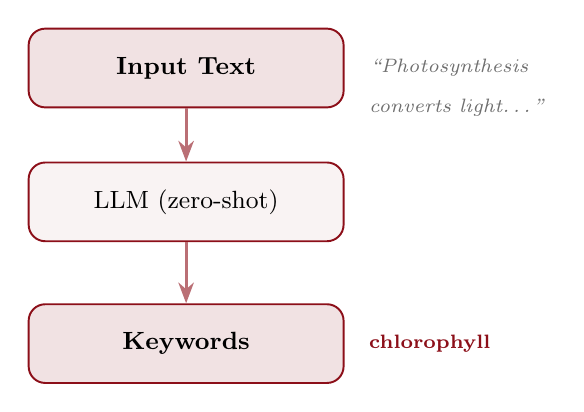
\begin{tikzpicture}[
        box/.style={draw=unisired, rounded corners=6pt, minimum width=4cm, minimum height=1cm, align=center, font=\small, fill=unisired!5, line width=0.7pt},
        arr/.style={->, >=Stealth, line width=1pt, unisired!60}
      ]
      \node[box, fill=unisired!12, font=\small\bfseries] (text) at (0, 3.5) {Input Text};
      \node[box] (llm) at (0, 1.8) {LLM (zero-shot)};
      \node[box, fill=unisired!12, font=\small\bfseries] (kw) at (0, 0) {Keywords};
      \draw[arr] (text) -- (llm);
      \draw[arr] (llm) -- (kw);

      \node[font=\scriptsize, text=graytext, right] at (2.2, 3.5) {\textit{``Photosynthesis}};
      \node[font=\scriptsize, text=graytext, right] at (2.2, 3.0) {\textit{converts light\ldots''}};
      \node[font=\scriptsize, text=unisired, right] at (2.2, 0) {\textbf{chlorophyll}};
      \end{tikzpicture}
  \end{columns}
  \vfill
  \centering
  {\small Result: $\approx$ \textbf{80\%} of extracted keywords rated suitable by evaluators.}
\end{frame}

% --- 3.3 Clue generation ---
\begin{frame}{Step 2: Clue Generation}
  \begin{columns}[c]
    \column{0.5\textwidth}
      \centering
      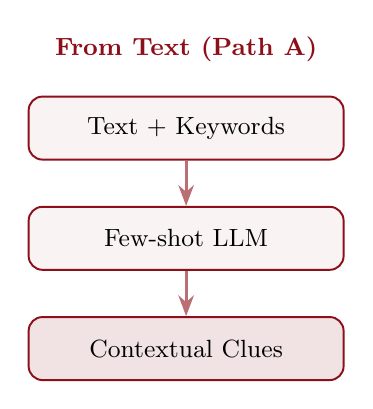
\begin{tikzpicture}[
        box/.style={draw=unisired, rounded corners=5pt, minimum width=4cm, minimum height=0.8cm, align=center, font=\small, fill=unisired!5, line width=0.7pt},
        arr/.style={->, >=Stealth, line width=1pt, unisired!60}
      ]
      \node[font=\small\bfseries, text=unisired] at (0, 4.2) {From Text (Path A)};
      \node[box] (ctx) at (0, 3.2) {Text + Keywords};
      \node[box] (fs) at (0, 1.8) {Few-shot LLM};
      \node[box, fill=unisired!12] (clue1) at (0, 0.4) {Contextual Clues};
      \draw[arr] (ctx) -- (fs);
      \draw[arr] (fs) -- (clue1);
      \end{tikzpicture}
    \column{0.5\textwidth}
      \centering
      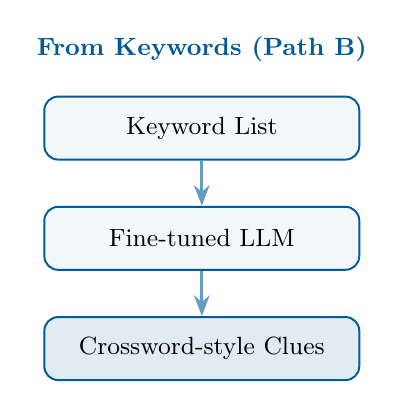
\begin{tikzpicture}[
        box/.style={draw=accentblue, rounded corners=5pt, minimum width=4cm, minimum height=0.8cm, align=center, font=\small, fill=accentblue!5, line width=0.7pt},
        arr/.style={->, >=Stealth, line width=1pt, accentblue!60}
      ]
      \node[font=\small\bfseries, text=accentblue] at (0, 4.2) {From Keywords (Path B)};
      \node[box] (kw) at (0, 3.2) {Keyword List};
      \node[box] (ft) at (0, 1.8) {Fine-tuned LLM};
      \node[box, fill=accentblue!12] (clue2) at (0, 0.4) {Crossword-style Clues};
      \draw[arr] (kw) -- (ft);
      \draw[arr] (ft) -- (clue2);
      \end{tikzpicture}
  \end{columns}
  \vfill
  \centering
  {\small From text: \textbf{70--77\%} acceptable \hspace{2em}
         From keywords: $\approx$ \textbf{60\%} with largest model}
\end{frame}

% --- 3.4 Grid generation ---
\begin{frame}{Step 3: Grid Generation}
  \begin{columns}[c]
    \column{0.55\textwidth}
      \small
      \textbf{Incremental greedy placement} with scoring:
      \vspace{0.4em}
      \begin{enumerate}
        \setlength\itemsep{0.4em}
        \item Start with the longest word
        \item For each remaining word, find\\
              the best intersection with placed words
        \item Score each candidate placement:
      \end{enumerate}
      \vspace{0.3em}
      \begin{equation*}
        S = \alpha \cdot I + \beta \cdot C - \gamma \cdot D
      \end{equation*}
      {\scriptsize\color{graytext} $I$ = intersections \quad $C$ = compactness \quad $D$ = density penalty}
      \vspace{0.4em}
      \begin{enumerate}
        \setcounter{enumi}{3}
        \item Stop when score degrades\\or all words are placed
      \end{enumerate}
    \column{0.45\textwidth}
      \centering
      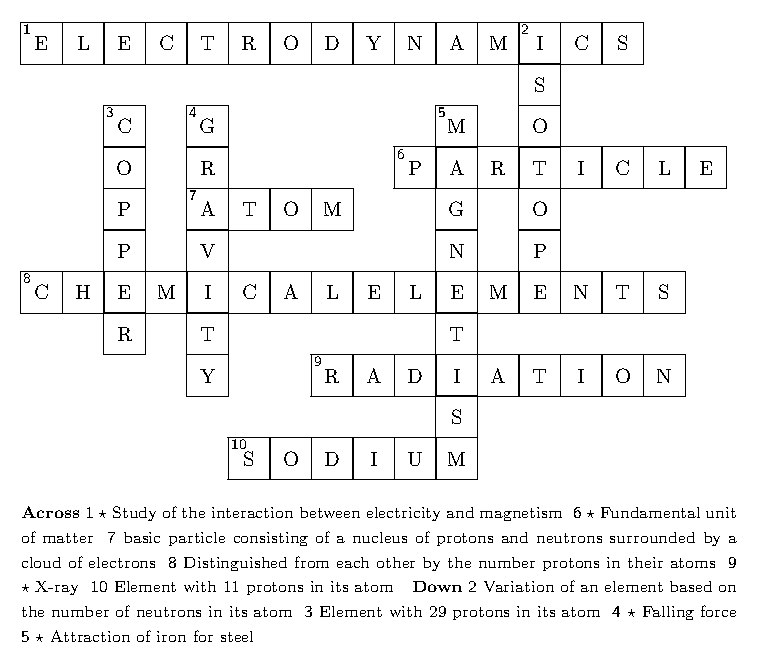
\includegraphics[width=0.78\textwidth]{figures/crossword.pdf}\\[0.5em]
      {\scriptsize\color{graytext} Example of a generated crossword grid}
  \end{columns}
\end{frame}

% --- 3.5 Results summary ---
\begin{frame}{End-to-End Evaluation}
  \vspace{0.5em}
  \begin{columns}[c]
    \column{0.33\textwidth}\centering
      \fcolorbox{unisired}{unisired!5}{\parbox{3cm}{\centering\vspace{0.4em}
      {\LARGE\color{unisired}\textbf{$\sim$80\%}}\\[0.2em]
      {\small Keyword\\Extraction\\Suitability}\vspace{0.4em}}}
    \column{0.33\textwidth}\centering
      \fcolorbox{unisired}{unisired!10}{\parbox{3cm}{\centering\vspace{0.4em}
      {\LARGE\color{unisired}\textbf{70--77\%}}\\[0.2em]
      {\small Acceptable\\Clues\\(from text)}\vspace{0.4em}}}
    \column{0.33\textwidth}\centering
      \fcolorbox{unisired}{unisired!15}{\parbox{3cm}{\centering\vspace{0.4em}
      {\LARGE\color{unisired}\textbf{$\sim$70\%}}\\[0.2em]
      {\small Flawed Clues\\Detected\\Automatically}\vspace{0.4em}}}
  \end{columns}
  \vfill
  \centering
  {\small Human-in-the-loop revision ensures final quality for classroom use.}
\end{frame}


% ======================================================
%  4 — SURPRISAL
% ======================================================
\section{Surprisal-Based Difficulty Modeling}

% --- 4.1 What is surprisal ---
\begin{frame}{What Is Surprisal?}
  \begin{columns}[c]
    \column{0.55\textwidth}
      \small
      From \textbf{information theory}:\\[0.5em]
      \begin{equation*}
        \text{Surprisal}(w_i) = -\log_2 P(w_i \mid w_1, \ldots, w_{i-1})
      \end{equation*}
      \vspace{0.8em}
      \textbf{Intuition:}\\[0.3em]
      \begin{itemize}
        \setlength\itemsep{0.5em}
        \item High surprisal $\rightarrow$ unexpected word $\rightarrow$ \textbf{harder}
        \item Low surprisal $\rightarrow$ predictable word $\rightarrow$ \textbf{easier}
      \end{itemize}
    \column{0.45\textwidth}
      \centering
      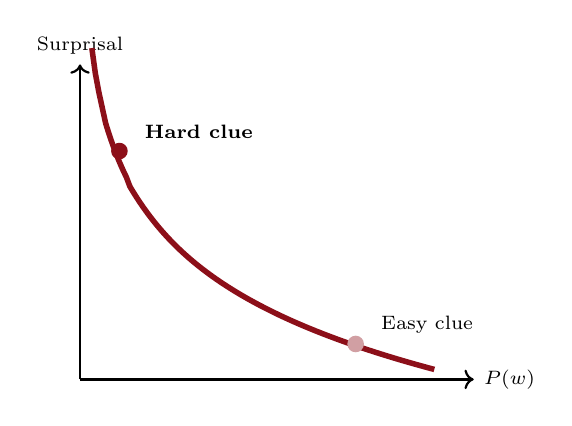
\begin{tikzpicture}
        \draw[->, thick] (0, 0) -- (5, 0) node[right, font=\scriptsize] {$P(w)$};
        \draw[->, thick] (0, 0) -- (0, 4) node[above, font=\scriptsize] {Surprisal};
        \draw[unisired, line width=2pt, domain=0.15:4.5, samples=100]
          plot (\x, {-1.2*ln(\x/5)});
        \fill[unisired] (0.5, 2.9) circle (3pt);
        \node[font=\scriptsize, right] at (0.7, 3.15) {\textbf{Hard clue}};
        \fill[unisired!40] (3.5, 0.45) circle (3pt);
        \node[font=\scriptsize, right] at (3.7, 0.7) {Easy clue};
      \end{tikzpicture}
  \end{columns}
\end{frame}

% --- 4.2 Key question ---
\begin{frame}{The Research Question}
  \begin{center}
    \vspace{1em}
    {\Large Can an LLM's \textbf{surprisal} predict\\[0.4em]
    how \textbf{difficult} a crossword clue is \textbf{for humans}?}
    \vspace{2em}

    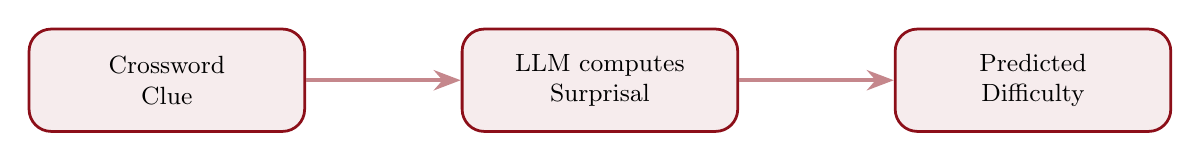
\begin{tikzpicture}[
      box/.style={draw=unisired, rounded corners=8pt, minimum width=3.5cm, minimum height=1.3cm, align=center, font=\small, line width=1pt},
      arr/.style={->, >=Stealth, line width=1.5pt, unisired!50}
    ]
    \node[box, fill=unisired!8] (clue) at (0, 0) {Crossword\\Clue};
    \node[box, fill=unisired!8] (llm) at (5.5, 0) {LLM computes\\Surprisal};
    \node[box, fill=unisired!8] (diff) at (11, 0) {Predicted\\Difficulty};
    \draw[arr] (clue) -- (llm);
    \draw[arr] (llm) -- (diff);
    \end{tikzpicture}

    \vspace{1.5em}
    {\small\color{graytext} If yes $\Rightarrow$ we can \textbf{automatically calibrate} puzzle difficulty\\
    to match the learner's level --- no human annotation needed.}
  \end{center}
\end{frame}

% --- 4.3 Results ---
\begin{frame}{Surprisal Correlates with Human Performance}
  \begin{columns}[c]
    \column{0.5\textwidth}
      \centering
      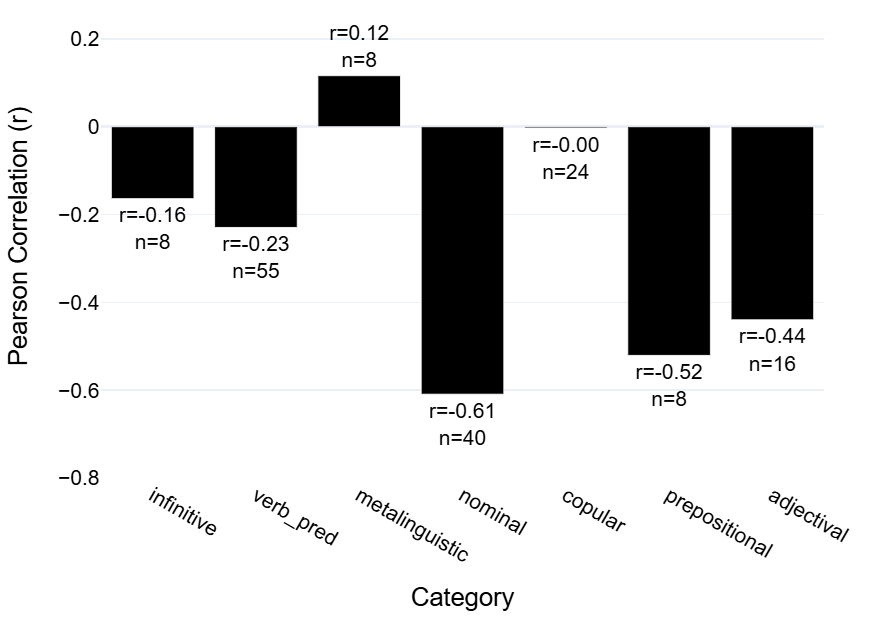
\includegraphics[width=\textwidth]{figures/accuracy-surprisal-macroGPT2.png}
    \column{0.5\textwidth}
      \begin{center}
        {\fontsize{38}{46}\selectfont\color{unisired}\textbf{$r \approx -0.57$}}\\[0.5em]
        {\large correlation with\\human accuracy}\\[1.5em]
        {\small Higher surprisal\\$\Rightarrow$ lower human accuracy}\\[1em]
        {\small\color{graytext} Effect is \textbf{stronger for nominal clues}\\
        (definition-style --- the most common type)}
      \end{center}
  \end{columns}
\end{frame}

% --- 4.4 Implications ---
\begin{frame}{Adaptive Difficulty for Education}
  \begin{center}
    \vspace{0.5em}
    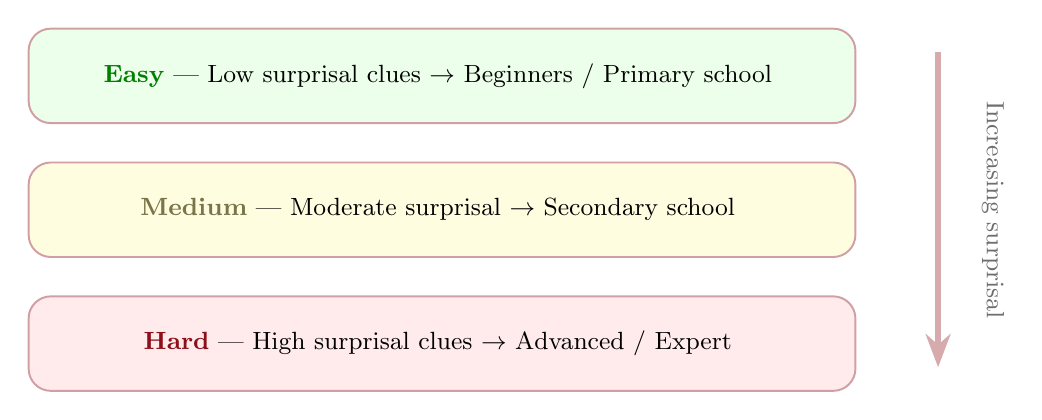
\begin{tikzpicture}[
      level/.style={draw=unisired!40, rounded corners=8pt, minimum width=10.5cm, minimum height=1.2cm, align=center, font=\small, line width=0.7pt},
    ]
    \node[level, fill=green!8] at (0, 2.5) {
      {\color{green!50!black}\textbf{Easy}} --- Low surprisal clues $\rightarrow$ Beginners / Primary school
    };
    \node[level, fill=yellow!12] at (0, 0.8) {
      {\color{yellow!40!black}\textbf{Medium}} --- Moderate surprisal $\rightarrow$ Secondary school
    };
    \node[level, fill=red!8] at (0, -0.9) {
      {\color{unisired}\textbf{Hard}} --- High surprisal clues $\rightarrow$ Advanced / Expert
    };
    \draw[->, >=Stealth, line width=2pt, unisired!35] (6.3, 2.8) -- (6.3, -1.2);
    \node[font=\small, text=graytext, rotate=-90] at (7, 0.8) {Increasing surprisal};
    \end{tikzpicture}

    \vspace{1.8em}
    {\large Surprisal enables \textbf{automatic difficulty calibration}\\[0.2em]
    without manual annotation.}
  \end{center}
\end{frame}


% ======================================================
%  5 — EDUCATIONAL IMPACT
% ======================================================
\section{Educational Impact}

\begin{frame}{Constructive AI Integration}
  \begin{columns}[c]
    \column{0.5\textwidth}
      \centering
      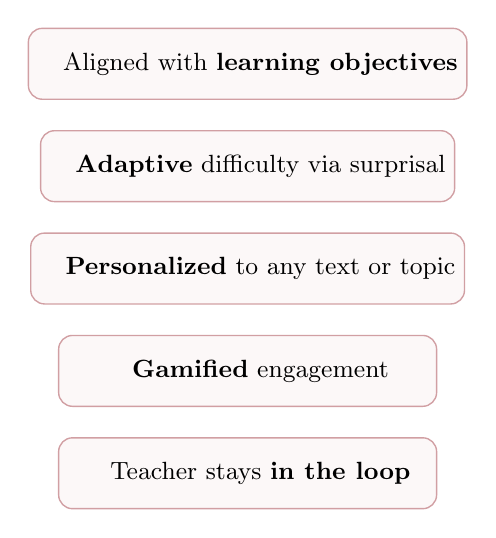
\begin{tikzpicture}[
        item/.style={draw=unisired!40, rounded corners=5pt, minimum width=4.8cm, minimum height=0.9cm, align=left, font=\small, fill=unisired!3, line width=0.5pt},
      ]
      \node[item] at (0, 3) {\quad Aligned with \textbf{learning objectives}};
      \node[item] at (0, 1.7) {\quad \textbf{Adaptive} difficulty via surprisal};
      \node[item] at (0, 0.4) {\quad \textbf{Personalized} to any text or topic};
      \node[item] at (0, -0.9) {\quad \textbf{Gamified} engagement};
      \node[item] at (0, -2.2) {\quad Teacher stays \textbf{in the loop}};
      \end{tikzpicture}
    \column{0.5\textwidth}
      \small
      The system embodies\\
      \textbf{constructive AI integration}:
      \vspace{0.5em}
      \begin{itemize}
        \setlength\itemsep{0.5em}
        \item AI \textit{supports} the teacher,\\doesn't replace them
        \item Crosswords from \textit{any text}\\or curriculum topic
        \item Active retrieval practice\\embedded in play
        \item Evidence-based: builds on\\proven gamification effects
      \end{itemize}
  \end{columns}
\end{frame}


% ======================================================
%  6 — YUKAI!
% ======================================================
\section{From Research to Product: Yukai!}

% --- 6.1 Intro + numbers ---
\begin{frame}{Yukai! --- University Spin-off}
  \begin{center}
    {\Large\color{unisired}\textbf{YUKAI!}}\\[0.2em]
    {\small Spin-off dell'Universit\`a di Siena per la Didattica Innovativa}\\[0.2em]
    {\scriptsize\color{graytext} \url{https://yukai.it} --- In partnership with Aret\`e Formazione}

    \vspace{1.2em}
    \begin{columns}[c]
      \column{0.25\textwidth}\centering
        \fcolorbox{unisired}{unisired!5}{\parbox{2.5cm}{\centering\vspace{0.3em}
        {\LARGE\color{unisired}\textbf{1,658}}\\[0.2em]
        {\scriptsize Crosswords\\Created}\vspace{0.3em}}}
      \column{0.25\textwidth}\centering
        \fcolorbox{unisired}{unisired!5}{\parbox{2.5cm}{\centering\vspace{0.3em}
        {\LARGE\color{unisired}\textbf{224}}\\[0.2em]
        {\scriptsize Educators\\Active}\vspace{0.3em}}}
      \column{0.25\textwidth}\centering
        \fcolorbox{unisired}{unisired!5}{\parbox{2.5cm}{\centering\vspace{0.3em}
        {\LARGE\color{unisired}\textbf{56}}\\[0.2em]
        {\scriptsize School\\Ambassadors}\vspace{0.3em}}}
      \column{0.25\textwidth}\centering
        \fcolorbox{unisired}{unisired!5}{\parbox{2.5cm}{\centering\vspace{0.3em}
        {\LARGE\color{unisired}\textbf{8,004}}\\[0.2em]
        {\scriptsize Learning\\Experiences}\vspace{0.3em}}}
    \end{columns}
  \end{center}
\end{frame}

% --- 6.2 How it works ---
\begin{frame}{1\ldots\, 2\ldots\, 3\ldots\, Yukai!}
  \vspace{1em}
  \begin{columns}[c]
    \column{0.3\textwidth}\centering
      \fcolorbox{unisired}{white}{\parbox{3.2cm}{\centering\vspace{0.5em}
      {\tikz\node[circle, fill=unisired, text=white, font=\bfseries, inner sep=2pt]{1};}\\[0.3em]
      \textbf{Create}\\[0.3em]
      {\scriptsize Enter topic or keywords ---\\AI generates the puzzle}
      \vspace{0.5em}}}
    \column{0.05\textwidth}\centering
      {\color{unisired}\Large$\rightarrow$}
    \column{0.3\textwidth}\centering
      \fcolorbox{unisired}{white}{\parbox{3.2cm}{\centering\vspace{0.5em}
      {\tikz\node[circle, fill=unisired, text=white, font=\bfseries, inner sep=2pt]{2};}\\[0.3em]
      \textbf{Customize}\\[0.3em]
      {\scriptsize Edit clues, answers,\\layout, difficulty level}
      \vspace{0.5em}}}
    \column{0.05\textwidth}\centering
      {\color{unisired}\Large$\rightarrow$}
    \column{0.3\textwidth}\centering
      \fcolorbox{unisired}{white}{\parbox{3.2cm}{\centering\vspace{0.5em}
      {\tikz\node[circle, fill=unisired, text=white, font=\bfseries, inner sep=2pt]{3};}\\[0.3em]
      \textbf{Share \& Play}\\[0.3em]
      {\scriptsize QR code or link ---\\any device, no account}
      \vspace{0.5em}}}
  \end{columns}
  \vfill
  \centering
  {\small\textbf{AI-powered creation} $\cdot$
  \textbf{Real-time analytics} $\cdot$
  \textbf{Multi-device} $\cdot$
  \textbf{No student accounts}}
\end{frame}

% --- 6.3 Features ---
\begin{frame}{Key Features}
  \begin{columns}[t]
    \column{0.33\textwidth}
      \centering
      {\color{unisired}\Large\textbf{For Teachers}}\\[0.8em]
      \small
      \begin{itemize}
        \setlength\itemsep{0.4em}
        \item AI generation in seconds
        \item Full customization
        \item Real-time student analytics
        \item Exportable results
      \end{itemize}
    \column{0.33\textwidth}
      \centering
      {\color{unisired}\Large\textbf{For Students}}\\[0.8em]
      \small
      \begin{itemize}
        \setlength\itemsep{0.4em}
        \item Play on any device
        \item No registration needed
        \item Contextual hints
        \item Engaging game format
      \end{itemize}
    \column{0.33\textwidth}
      \centering
      {\color{unisired}\Large\textbf{For Schools}}\\[0.8em]
      \small
      \begin{itemize}
        \setlength\itemsep{0.4em}
        \item Ambassador network
        \item Partnership with\\Aret\`e Formazione
        \item Presented at Didacta 2026
        \item LMS integration (beta)
      \end{itemize}
  \end{columns}
\end{frame}


% ======================================================
%  7 — CONCLUSIONS
% ======================================================
\section{Conclusions}

\begin{frame}{Contributions}
  \begin{enumerate}
    \setlength\itemsep{0.7em}
    \item \textbf{125,600-pair dataset} with 20+ syntactic categories\\
          {\scriptsize\color{graytext} Largest Italian crossword linguistic resource --- publicly available}

    \item \textbf{End-to-end generation pipeline}\\
          {\scriptsize\color{graytext} Text or keywords $\rightarrow$ validated clues $\rightarrow$ crossword grid}

    \item \textbf{Surprisal-based difficulty model}\\
          {\scriptsize\color{graytext} $r \approx -0.57$ with human accuracy --- enables adaptive calibration}

    \item \textbf{Yukai! spin-off} --- from research to real classrooms\\
          {\scriptsize\color{graytext} 1,658 crosswords $\cdot$ 224 educators $\cdot$ 8,004 learning experiences}
  \end{enumerate}
\end{frame}

\begin{frame}{Publications}
  \small
  \begin{enumerate}
    \setlength\itemsep{0.55em}
    \item \textbf{IJCOL 2025} --- Italian Crossword Generator: In-depth Linguistic Analysis
    \item \textbf{ICMLA 2023} --- Building Bridges of Knowledge: Automated Crossword Generation
    \item \textbf{CLiC-it 2023} --- Italian Crossword Generator: Interactive Word Puzzles
    \item \textbf{INTETAIN 2023} --- The WebCrow French Crossword Solver
    \item \textbf{CLiC-it 2025} \textit{(accepted)} --- Surprisal and Crossword Clues Difficulty
  \end{enumerate}
\end{frame}


% ======================================================
%  THANK YOU
% ======================================================
{
\setbeamertemplate{footline}{}
\setbeamercolor{background canvas}{bg=unisired}
\begin{frame}[plain]
  \vfill
  \begin{center}
    {\fontsize{34}{40}\selectfont\color{white}\textbf{Thank you!}}\\[1em]
    {\large\color{white!80} Questions?}\\[0.6em]
    {\small\color{white!60}\textit{I hope this wasn't too\ldots\ puzzling.}}\\[2em]
    {\small\color{white!60} Tommaso Iaquinta $\cdot$ tommaso.iaquinta@unisi.it}\\[0.3em]
    {\small\color{white!60} \url{https://yukai.it}}
  \end{center}
  \vfill
\end{frame}
}

\end{document}